%HW02.tex
%
% Second Homework for Graduate Algebra
% Frank Sottile
%%%%%%%%%%%%%%%%%%%%%%%%%%%%%%%%%%%%%%%%%%%%%%%%%%%%%%%%%%%%%%%%%%%%%%%
\documentclass[12pt]{article}
\usepackage{multicol,amsfonts, amssymb,  mathtools,amsmath}
\usepackage{colordvi,graphicx}
\headheight=8pt
%
\topmargin=-75pt
\textheight=720pt   \textwidth=560pt
\oddsidemargin=-60pt \evensidemargin=-60pt

\pagestyle{empty}

%%%%%%%%%%%%%%%%%%%%%%%%%%%%%%%%%%%%%%%%%%%%
\newcommand{\CC}{{\mathbb C}}
\newcommand{\KK}{{\mathbb K}}
\newcommand{\NN}{{\mathbb N}}
\newcommand{\QQ}{{\mathbb Q}}
\newcommand{\RR}{{\mathbb R}}
\newcommand{\TT}{{\mathbb T}}
\newcommand{\ZZ}{{\mathbb Z}}

\newcommand{\calA}{{\mathcal A}}
\newcommand{\be}{{\bf e}}
\newcommand{\bfi}{{\bf i}}
\newcommand{\bfj}{{\bf j}}

\newcommand{\Hom}{\mbox{Hom}}
\newcommand{\spec}{\mbox{spec}}
\newcommand{\cone}{\mbox{cone}}

\newcommand{\vect}[2]{(\begin{smallmatrix}#1\\#2\end{smallmatrix})}
\newcommand{\msp}{\hspace{8pt}}
%\newcommand{\Square}{\raisebox{-2pt}{\includegraphics{images/Square.eps}}}
\newcommand{\Square}{\raisebox{-2pt}{\Large$\square$}}

\def\Color#1#2{\special{color push cmyk #1}#2\special{color pop}}
%\def\Indigo#1{\Color{.42 1. 0. .49}{#1}}
\def\Indigo#1{\Color{1. .95 .05 .4}{#1}}
\def\MyViolet#1{\Color{.6 1. 0. .15}{#1}}
\def\TAMU#1{\Color{.15 1. .39 .69}{#1}}

\newcommand{\barsl}{\noindent\begin{minipage}[t]{590pt}
\Indigo{\rule{590pt}{1.2pt}}\vspace{-5.7mm}\\
\MyViolet{\rule{590pt}{1.2pt}}\vspace{-5.7mm}\\
\Blue{\rule{590pt}{1.2pt}}\vspace{-5.7mm}\\
\Green{\rule{590pt}{1.2pt}}\vspace{-5.7mm}\\
\Yellow{\rule{590pt}{1.2pt}}\vspace{-5.7mm}\\
\Orange{\rule{590pt}{1.2pt}}\vspace{-5.7mm}\\
\Red{\rule{590pt}{1.2pt}}\bigskip
\end{minipage}}


\newcommand{\barsn}{\noindent\begin{minipage}[t]{590pt}
\Indigo{\rule{590pt}{1.1pt}}\vspace{-4.5mm}\\
\MyViolet{\rule{590pt}{1.1pt}}\vspace{-4.5mm}\\
\Blue{\rule{590pt}{1.1pt}}\vspace{-4.5mm}\\
\Green{\rule{590pt}{1.1pt}}\vspace{-4.5mm}\\
\Yellow{\rule{590pt}{1.1pt}}\vspace{-4.5mm}\\
\Orange{\rule{590pt}{1.1pt}}\vspace{-4.5mm}\\
\Red{\rule{590pt}{1.1pt}}\bigskip
\end{minipage}}

\def\demph#1{\TAMU{{\sl #1}}}
\def\defcolor#1{\TAMU{#1}}

\begin{document}
\LARGE 
\noindent
Algebra \ \ Autumn 2025\vspace{1pt}\\
Frank Sottile\vspace{2pt}\\
\Large 29 August 2025 \hfill
\sf
 Second Homework\makebox[20pt][l]{\ }
\normalsize\vspace{10pt}

\noindent
Write your answers neatly, in complete sentences.  
I highly recommend recopying your work before handing it in.
Correct and crisp proofs are greatly appreciated; oftentimes your work can be shortened and made clearer.

The last two problems were partially done in class.
This is an opportunity to polish your skills at writing mathematics in a clear and organized manner.

\barsn

\noindent\Maroon{{\sf Hand in at the start of class, Thursday 4 September:}} 

\begin{enumerate}

%%%%%%%%%%%%%%%%%%%%%%%%%%%%%%%%%%%%%%%%%%%%%%%%%%%%%%%%%%%%%%%%%%%%%%%%%%%%%%%%%%%%%%%%%%%%%%%%%%%%
\item  Let $G$ be a group, $H$ be a subgroup of $G$, and $g\in G$.
       Prove that $gHg^{-1}$ is a subgroup of $G$ and that it is isomorphich to $H$.
%%%%%%%%%%%%%%%%%%%%%%%%%%%%%%%%%%%%%%%%%%%%%%%%%%%%%%%%%%%%%%%%%%%%%%%%%%%%%%%%%%%%%%%%%%%%%%%%%%%%

 
%%%%%%%%%%%%%%%%%%%%%%%%%%%%%%%%%%%%%%%%%%%%%%%%%%%%%%%%%%%%%%%%%%%%%%%%%%%%%%%%%%%%%%%%%%%%%%%%%%%%
\item      Show that a group $G$ cannot be the union of two proper subgroups.

  
  Show that the additive group of ordered pairs of integers $\ZZ\oplus\ZZ$ is the union of three proper subgroups,
  by exhibiting three such subgroups.
%%%%%%%%%%%%%%%%%%%%%%%%%%%%%%%%%%%%%%%%%%%%%%%%%%%%%%%%%%%%%%%%%%%%%%%%%%%%%%%%%%%%%%%%%%%%%%%%%%%%
 


 
%%%%%%%%%%%%%%%%%%%%%%%%%%%%%%%%%%%%%%%%%%%%%%%%%%%%%%%%%%%%%%%%%%%%%%%%%%%%%%%%%%%%%%%%%%%%%%%%%%%%
\item Let $A,B$ be groups with elements $a\in A$ and $b\in B$.
      What is the order of the element $(a,b)\in A\times B$?
%%%%%%%%%%%%%%%%%%%%%%%%%%%%%%%%%%%%%%%%%%%%%%%%%%%%%%%%%%%%%%%%%%%%%%%%%%%%%%%%%%%%%%%%%%%%%%%%%%%%


%%%%%%%%%%%%%%%%%%%%%%%%%%%%%%%%%%%%%%%%%%%%%%%%%%%%%%%%%%%%%%%%%%%%%%%%%%%%%%%%%%%%%%%%%%%%%%%%%%
\item Assume that $G=\{e,a,b,c\}$ is a group with four elements and identity $e$.
      Suppose that $G$ has no element of order four.
      Prove that there is a unique group structure for $G$ and deduce that $G$ is  abelian.
      What is the case if $G$ has an element of oder $4$?
%%%%%%%%%%%%%%%%%%%%%%%%%%%%%%%%%%%%%%%%%%%%%%%%%%%%%%%%%%%%%%%%%%%%%%%%%%%%%%%%%%%%%%%%%%%%%%%%%%%%


%%%%%%%%%%%%%%%%%%%%%%%%%%%%%%%%%%%%%%%%%%%%%%%%%%%%%%%%%%%%%%%%%%%%%%%%%%%%%%%%%%%%%%%%%%%%%%%%%%%%
\item 
    Prove that every finitely generated subgroup of the rational numbers $\QQ$ is cyclic.
      Give an example (with proof) of a subgroup of $\QQ$ that is not finitely generated.
%%%%%%%%%%%%%%%%%%%%%%%%%%%%%%%%%%%%%%%%%%%%%%%%%%%%%%%%%%%%%%%%%%%%%%%%%%%%%%%%%%%%%%%%%%%%%%%%%%%%  





%%%%%%%%%%%%%%%%%%%%%%%%%%%%%%%%%%%%%%%%%%%%%%%%%%%%%%%%%%%%%%%%%%%%%%%%%%%%%%%%%%%%%%%%%%%%%%%%%%%%
% 
\item 
    Let \defcolor{$D_4$} be the group under matrix multiplication generated by the real $2\times 2$ matrices 
      $\defcolor{S}:=\vect{\msp 0&1}{-1&0}$ and $\defcolor{R}:=\vect{0&1}{1&0}$.
      Show that $D_4$ is a nonabelian group of order $8$.

      Let $\Square$ be the square with vertices $(\pm1,\pm1)$ in $\RR^2$.
      Show that $D_4$ acts on $\Square$, and is its group of symmetries, called the \demph{dihedral group} of order  8.
%%%%%%%%%%%%%%%%%%%%%%%%%%%%%%%%%%%%%%%%%%%%%%%%%%%%%%%%%%%%%%%%%%%%%%%%%%%%%%%%%%%%%%%%%%%%%%%%%%%%

%%%%%%%%%%%%%%%%%%%%%%%%%%%%%%%%%%%%%%%%%%%%%%%%%%%%%%%%%%%%%%%%%%%%%%%%%%%%%%%%%%%%%%%%%%%%%%%%%%%%
\item 
    Let \defcolor{$Q_8$} be the group generated by the complex $2\times 2$ matrices 
      $\defcolor{\bfi}:=\vect{\msp 0&1}{-1&0}$ and $\defcolor{\bfj}:=\vect{0&\sqrt{-1}}{\sqrt{-1}&0}$.
      Show that $Q_8$ is a nonabelian group of order $8$. 
      Hint: Observe that $\bfi\bfj=\bfj\bfi^3$, so that every element of $Q_8$ has the form $\bfi^a\bfj^b$.
        Note further that $\bfi^4=\bfj^4=\vect{1&0}{0&1}$, the identity.
      This is the \demph{quaternion} group.

      Comparing subgroups, or the number of elements of different orders, show that $Q_8$ is not isomorphic to $D_4$.
%%%%%%%%%%%%%%%%%%%%%%%%%%%%%%%%%%%%%%%%%%%%%%%%%%%%%%%%%%%%%%%%%%%%%%%%%%%%%%%%%%%%%%%%%%%%%%%%%%%%  




      
\end{enumerate}
%%%%%%%%%%%%%%%%%%%%%%%%%%%%%%%%%%%%%%%%%%%%%%%%%%%%%%%%%%%%%%%%%%%%%%%%%%%%%%%%%%%%%%%%%%%%%%%%%%%%

\end{document}
